% Choose one to switch between slides and handout
\documentclass[]{beamer}
%\documentclass[handout]{beamer}

% Video Meta Data
\title{Smart Contracts and Decentralized Finance Applications}
\subtitle{Title of Video Lecture}
\author{Prof. Dr. Fabian Schär}
\institute{University of Basel}

% Config File
% Packages
\usepackage[utf8]{inputenc}
\usepackage{hyperref}
\usepackage{gitinfo2}
\usepackage{tikz}
 \usetikzlibrary{calc}
\usepackage{amsmath}
\usepackage{mathtools}
\usepackage{bibentry}
\usepackage{xcolor}
\usepackage{colortbl} % Add colour to LaTeX tables
\usepackage{caption}
\usepackage[export]{adjustbox}
\usepackage{pgfplots} \pgfplotsset{compat = 1.17}
\usepackage{makecell}
\usepackage{fancybox}
\usepackage{ragged2e}
\usepackage{fontawesome}
\usepackage{seqsplit}
\usepackage{tabularx}
\usepackage{tcolorbox}
\usepackage{booktabs} % use instead  \hline in tables

% Color Options
\definecolor{highlight}{rgb}{0.65,0.84,0.82}
\definecolor{focus}{rgb}{0.72, 0, 0}
\definecolor{lightred}{rgb}{0.8,0.5,0.5}
\definecolor{midgray}{RGB}{190,195,200}

 %UniBas Main Colors
\definecolor{mint}{RGB}{165,215,210}
\definecolor{anthracite}{RGB}{45,55,60}
\definecolor{red}{RGB}{210,5,55}

 %UniBas Color Palette (for graphics)
\definecolor{strongmint}{RGB}{30,165,165}
\definecolor{darkmint}{RGB}{0,110,110}
\definecolor{softanthracite}{RGB}{140,145,150}
\definecolor{brightanthracite}{RGB}{190,195,200}
\definecolor{softred}{RGB}{235,130,155}

%Custom Colors
\definecolor{lightergray}{RGB}{230, 230, 230}



% Beamer Template Options
\beamertemplatenavigationsymbolsempty
\setbeamertemplate{footline}[frame number]
\setbeamercolor{structure}{fg=black}
\setbeamercolor{footline}{fg=black}
\setbeamercolor{title}{fg=black}
\setbeamercolor{frametitle}{fg=black}
\setbeamercolor{item}{fg=black}
\setbeamercolor{}{fg=black}
\setbeamercolor{bibliography item}{fg=black}
\setbeamercolor*{bibliography entry title}{fg=black}
\setbeamercolor{alerted text}{fg=focus}
\setbeamertemplate{items}[square]
\setbeamertemplate{enumerate items}[default]
\captionsetup[figure]{labelfont={color=black},font={color=black}}
\captionsetup[table]{labelfont={color=black},font={color=black}}

\setbeamertemplate{bibliography item}{\insertbiblabel}

%tcolor boxes
\newtcolorbox{samplecode}[2][]{
  colback=mint, colframe=darkmint, coltitle=white,
  fontupper = \ttfamily\scriptsize, fonttitle= \bfseries\scriptsize,
  boxrule = 0mm, arc = 0mm,
  boxsep = 1.3mm, left = 0mm, right = 0mm, top = 0.5mm, bottom = 0mm, middle=0mm,
  #1,title=#2}
  
\newtcolorbox{keytakeaway}[2][]{
  colback=softred, colframe=red, coltitle=white,
  fontupper = \scriptsize, fonttitle= \bfseries\scriptsize,
  boxrule = 0mm, arc = 0mm,
  boxsep = 1.3mm, left = 0mm, right = 0mm, top = 0.5mm, bottom = 0mm, middle=0mm,
  #1,title=#2}

\newtcolorbox{exercise}[2][]{
  colback=brightanthracite, colframe=anthracite, coltitle=white,
  fontupper = \scriptsize, fonttitle= \bfseries\scriptsize,
  boxrule = 0mm, arc = 0mm,
  boxsep = 1.3mm, left = 0mm, right = 0mm, top = 0.5mm, bottom = 0mm, middle=0mm,
  #1,title=#2}



% Link Icon Command 
\newcommand{\link}{%
    \tikz[x=1.2ex, y=1.2ex, baseline=-0.05ex]{%
        \begin{scope}[x=1ex, y=1ex]
            \clip (-0.1,-0.1)
                --++ (-0, 1.2)
                --++ (0.6, 0)
                --++ (0, -0.6)
                --++ (0.6, 0)
                --++ (0, -1);
            \path[draw,
                line width = 0.5,
                rounded corners=0.5]
                (0,0) rectangle (1,1);
        \end{scope}
        \path[draw, line width = 0.5] (0.5, 0.5)
            -- (1, 1);
        \path[draw, line width = 0.5] (0.6, 1)
            -- (1, 1) -- (1, 0.6);
        }
    }

% Other commands
\newcommand\tab[1][0.5cm]{\hspace*{#1}} % for code boxes


% Read Git Data from Github Actions Workflow
% Defaults to gitinfo2 for local builds
\IfFileExists{gitInfo.txt}
	{\input{gitInfo.txt}}
	{
		\newcommand{\gitRelease}{(Local Release)}
		\newcommand{\gitSHA}{\gitHash}
		\newcommand{\gitDate}{\gitAuthorIsoDate}
	}

% Custom Titlepage
\defbeamertemplate*{title page}{customized}[1][]
{
  \vspace{-0cm}\hfill\includegraphics[width=2.5cm]{../config/logo_cif}
  \includegraphics[width=1.9cm]{../config/seal_wwz}
  \\ \vspace{2em}
  \usebeamerfont{title}\textbf{\inserttitle}\par
  \usebeamerfont{title}\usebeamercolor[fg]{title}\insertsubtitle\par  \vspace{1.5em}
  \small\usebeamerfont{author}\insertauthor\par
  \usebeamerfont{author}\insertinstitute\par \vspace{2em}
  \usebeamercolor[fg]{titlegraphic}\inserttitlegraphic
    \tiny \noindent \texttt{Release Ver.: \gitRelease}\\ 
    \texttt{Version Hash: \gitSHA}\\
    \texttt{Version Date: \gitDate}\\ \vspace{1em}
    
    
    \iffalse
  \link \href{https://github.com/cifunibas/Bitcoin-Blockchain-Cryptoassets/blob/main/slides/intro.pdf}
  {Get most recent version}\\
  \link \href{https://github.com/cifunibas/Bitcoin-Blockchain-Cryptoassets/blob/main/slides/intro.pdf}
  {Watch video lecture}\\ 
  
  \fi
  
  \vspace{1em}
  License: \texttt{Creative Commons Attribution-NonCommercial-ShareAlike 4.0 International}\\\vspace{2em}
  \includegraphics[width = 1.2cm]{../config/license}
}


% tikzlibraries
\usetikzlibrary{decorations.pathreplacing}
\usetikzlibrary{decorations.markings}
\usetikzlibrary{positioning}
\usetikzlibrary{calc}
\captionsetup{font=footnotesize}

%%%%%%%%%%%%%%%%%%%%%%%%%%%%%%%%%%%%%%%%%%%%%%
%%%%%%%%%%%%%%%%%%%%%%%%%%%%%%%%%%%%%%%%%%%%%%
\begin{document}

\thispagestyle{empty}
\begin{frame}[noframenumbering]
	\titlepage
\end{frame}

%%%

\begin{frame}{Blockchain Origin}

\centering
\includegraphics[width = 5cm, frame]{../assets/images/nakamoto_cover}
		
\textbf{Bitcoin: A Peer-to-Peer Electronic Cash System} \\ 
Satoshi Nakamoto \\
\link \href{https://bitcoin.org/bitcoin.pdf}{Online version}

\end{frame}
%%%

%%%
\begin{frame}{Payment Systems: Today's Challenge}

Physical Cash: Presence in the same place at the same time
\begin{figure}[h]
	\center
		\input{../assets/figures/cash_payment.tex}
\end{figure}

\vspace{1.5 em}

\uncover<2->{Digital Cash: Proof of ownership
\begin{figure}[h]
	\center
		\input{../assets/figures/ecash_payment.tex}
\end{figure}}
	
\end{frame}
%%%	


%%%
\begin{frame}{Today's Solution: Intermediaries Keeping Money Registries}

\begin{figure}[h]
	\center
		\input{../assets/figures/registry_payment.tex}
\end{figure}

\uncover<2->{\vspace{1 em}

\textbf{Registry Types}\\
\vspace{1 em}
\textbf{Implicit:} Verbal agreements, limited to small groups.\\
\textbf{Explicit:} Records in written or digital databases.}
	
\end{frame}
%%%	


%%%
\begin{frame}{Implicit Registry Example: The Stone Money of Yap}
	\center
	\includegraphics[width=8cm]{../assets/images/yap_stones}\\
	\footnotesize{Picture source: Eric Guinther}
\end{frame}
%%%


%%%
\begin{frame}{Implicit Registry Example: The Stone Money of Yap}

\begin{figure}[h]
	\center
		\input{../assets/figures/yap_system.tex}
\end{figure}
	
\end{frame}
%%%

%%%
\begin{frame}{Scaling the Yap Network}
	\begin{figure}
			\input{../assets/figures/yap_network.tex}
	\end{figure}
	\vspace{1em}
	\uncover<4->{
		\textbf{Large network size results in three problems:}
		\begin{itemize}
			\item<5-> Transaction capacity
			\item<6-> Transaction legitimacy
			\item<7-> Transaction consensus
		\end{itemize}
	}
	\vspace{1em}
	
\uncover<8->{
	\begin{alertblock}{Key idea}
		Blockchains as decentralized data structures that are maintained by its participants in the absence of a centralized third party. 	
	\end{alertblock}
}
\end{frame}
%%%


%%%
\begin{frame}{Transaction Capacity}
\textbf{Goal:} Ensure that each participant can reliably \color{focus}initiate a transaction \color{black} without having to fear censorship. \\
\uncover<2->{
	\begin{figure}[h!]
		\center
		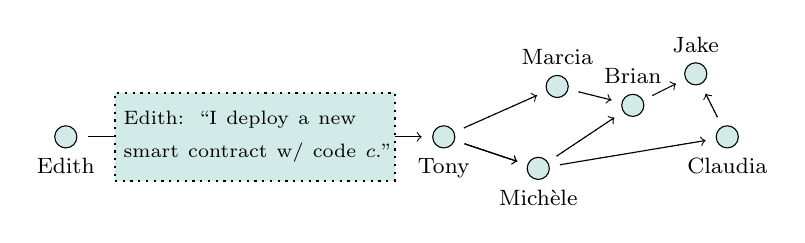
\begin{tikzpicture}[domain=-8:8, scale=0.8]

% transaction
\uncover<3->{
	\coordinate (c1) at (0,0);
	\coordinate (c2) at (6,0);
	\filldraw[draw=black,fill=highlight!50] (c1) circle (5pt) node[below=0.15cm,color=black]{\footnotesize{Edith}};
	\draw[shorten >=0.28cm,shorten <=0.28cm,->] (c1) to[] (c2);
}

% network
\uncover<2->{
\coordinate (c3) at (7.8,0.8);
\coordinate (c4) at (7.5,-0.5);
\coordinate (c5) at (9,0.5);
\coordinate (c6) at (10,1);
\coordinate (c7) at (10.5,0);
\filldraw[draw=black,fill=highlight!50] (c2) circle (5pt) node[below=0.15cm,color=black]{\footnotesize{Tony}};
\filldraw[draw=black,fill=highlight!50] (c3) circle (5pt) node[above=0.15cm,color=black]{\footnotesize{Marcia}};
\filldraw[draw=black,fill=highlight!50] (c4) circle (5pt) node[below=0.15cm,color=black]{\footnotesize{Michèle}};
\filldraw[draw=black,fill=highlight!50] (c5) circle (5pt) node[above=0.15cm,color=black]{\footnotesize{Brian}};
\filldraw[draw=black,fill=highlight!50] (c6) circle (5pt) node[above=0.15cm,color=black]{\footnotesize{Jake}};
\filldraw[draw=black,fill=highlight!50] (c7) circle (5pt) node[below=0.15cm,color=black]{\footnotesize{Claudia}};
}

\uncover<3->{
\draw[shorten >=0.28cm,shorten <=0.28cm,->] (c2) to[] (c3);
\draw[shorten >=0.28cm,shorten <=0.28cm,->] (c2) to[] (c4);
\draw[shorten >=0.28cm,shorten <=0.28cm,->] (c2) to[] (c4);
\draw[shorten >=0.28cm,shorten <=0.28cm,->] (c3) to[] (c5);
\draw[shorten >=0.28cm,shorten <=0.28cm,->] (c4) to[] (c5);
\draw[shorten >=0.28cm,shorten <=0.28cm,->] (c4) to[] (c7);
\draw[shorten >=0.28cm,shorten <=0.28cm,->] (c5) to[] (c6);
\draw[shorten >=0.28cm,shorten <=0.28cm,->] (c7) to[] (c6);
}

\uncover<2>{
\draw[shorten >=0.28cm,shorten <=0.28cm, dotted] (c2) to[] (c3);
\draw[shorten >=0.28cm,shorten <=0.28cm, dotted] (c2) to[] (c4);
\draw[shorten >=0.28cm,shorten <=0.28cm, dotted] (c2) to[] (c4);
\draw[shorten >=0.28cm,shorten <=0.28cm, dotted] (c3) to[] (c5);
\draw[shorten >=0.28cm,shorten <=0.28cm, dotted] (c4) to[] (c5);
\draw[shorten >=0.28cm,shorten <=0.28cm, dotted] (c4) to[] (c7);
\draw[shorten >=0.28cm,shorten <=0.28cm, dotted] (c5) to[] (c6);
\draw[shorten >=0.28cm,shorten <=0.28cm, dotted] (c7) to[] (c6);
}

% value transaction
\uncover<3>{
\filldraw[fill=highlight!50,dotted,thick] (0.78,-0.7) -- (5.22,-0.7) -- (5.22,0.7) -- (0.78,0.7) -- (0.78,-0.7) node[midway, right=-0.02cm,text width=4.25cm]{\scriptsize{Edith: ``I transfer one \\ Ether to Daniel.''}};
}

% smart contract interaction
\uncover<4>{
\filldraw[fill=highlight!50,dotted,thick] (0.78,-0.7) -- (5.22,-0.7) -- (5.22,0.7) -- (0.78,0.7) -- (0.78,-0.7) node[midway, right=-0.02cm,text width=4.25cm]{\scriptsize{Edith: ``Execute function \\ $f$ of \texttt{0x...} with data $d$.''}};
}

% smart contract deployment
\uncover<5>{
\filldraw[fill=highlight!50,dotted,thick] (0.78,-0.7) -- (5.22,-0.7) -- (5.22,0.7) -- (0.78,0.7) -- (0.78,-0.7) node[midway, right=-0.02cm,text width=4.25cm]{\scriptsize{Edith: ``I deploy a new \\ smart contract w/ code $c$.''}};
}


\end{tikzpicture}

	\end{figure}\vspace{1em}
}
\uncover<2->{
	Peer-to-Peer Network:
        \begin{itemize}
		\item<1-> Permissionless
		\item<1-> Censorship-resistant
		\item<1-> No special privileges
		\end{itemize}
		}
\end{frame}
%%%

%%%
\begin{frame}{Centralized vs. Decentralized Networks}

	\begin{columns}[T]
		\begin{column}{0.5\textwidth}
		\center
			\begin{tikzpicture}[scale=0.56, every node/.style={scale=0.63}]
				\input{../assets/figures/centralized_network}
			\end{tikzpicture}
		\end{column}
		\begin{column}{0.5\textwidth}
		\center
			\begin{tikzpicture}[scale=0.63, every node/.style={scale=0.63}]
				\input{../assets/figures/p2p}
			\end{tikzpicture}
		\end{column}
	\end{columns}
	
	\vspace{1em}
	\begin{columns}[T]
		\begin{column}{0.5\textwidth}
		\center
		\textbf{Centralized}
		\end{column}
		\begin{column}{0.5\textwidth}
		\center
		\textbf{Decentralized}
		\end{column}
		
	\end{columns}
		
	
\end{frame}
%%%

%%%
\begin{frame}{Personal Database and Transaction Queue}
	\begin{minipage}{0.15\textwidth}
		\center
		\includegraphics[width=2.4cm]{../assets/images/miner_single.png}
	\end{minipage}
	\begin{minipage}{0.1\textwidth}
		
\begin{tikzpicture}[scale=1]
			\draw [decorate,decoration={brace,amplitude=10pt}, color = mint, line width=2pt]
			(0.5,0.0) -- (0.5,5.5) node [black,midway,xshift=-0.8cm] 
			{\footnotesize};
		\end{tikzpicture}
	\end{minipage}
	\begin{minipage}{0.7\textwidth}
		\uncover<1->{\textbf{Personal Version of the Blockchain}}
		\begin{itemize}
			\item<1-> Personal ledger of valid transactions in block structure.
			\item<1-> Has an incentive to keep in sync with consensus.
		\end{itemize}
		\vspace{1em}
		\uncover<2->{\textbf{Personal Transaction Queue}}
		\begin{itemize}
			\item<2-> Transactions that are not yet valid.
			\item<2-> Waiting for inclusion in database $\rightarrow$ queue.
		\end{itemize}
	\end{minipage}

	
\end{frame}
%%%	

%%%
\begin{frame}{Handshake and Address List}
	\vspace{1em}
	\begin{center}
		\begin{tikzpicture}[scale=0.7, every node/.style={scale=0.7}]
			\input{../assets/figures/ver_verack}
		\end{tikzpicture}
	\end{center}
	
	\vspace{0.5em}

	\begin{center}
		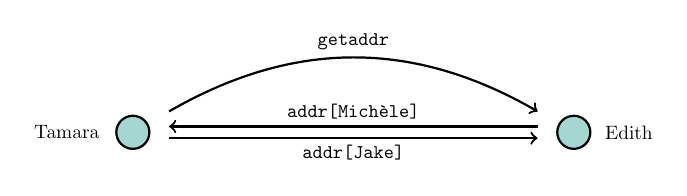
\begin{tikzpicture}[scale=0.7, every node/.style={scale=0.7}]
			%Set Anchor Points
		
\coordinate (1) at (-4, 0);
\coordinate (2) at (4, 0);

\node(node1)[minimum size = 1.3cm] at (1) {};
\node(node2)[minimum size = 1.3cm] at (2) {};

%Tamara and Edith

\node(node3)[xshift = -1.2cm] at (1) {Tamara};
\node(node4)[xshift = 1cm] at (2) {Edith};


\filldraw[fill=highlight, thick](1) circle (.3);
\filldraw[fill=highlight, thick](2) circle (.3);

%Interactions

\draw[->, thick] (node1) edge [out=30, in=-210] node[midway,above] {\texttt{getaddr}} (node2);
\draw[<-, thick] ([yshift=3pt]node1.east) -- node[midway,above] {\texttt{addr[Michèle]}} ([yshift=3pt]node2.west);
\draw[->, thick] ([yshift=-3pt]node1.east) -- node[midway,below] {\texttt{addr[Jake]}} ([yshift=-3pt]node2.west);
		\end{tikzpicture}	
	\end{center}
	
	\vspace{0.25em}

	\begin{center}
		\begin{tikzpicture}[scale=0.72, every node/.style ={scale=0.8}]
			\input{../assets/figures/network_with_computing_power}
		\end{tikzpicture}
	\end{center}
\end{frame}
%%%

%%%
\begin{frame}{Exchange of Blocks and Transactions}

	\begin{center}
		\begin{tikzpicture}[scale=0.7, every node/.style={scale=0.7}]
			\input{../assets/figures/block_exchange}
		\end{tikzpicture}
	\end{center}
	\vspace{1em}
	\begin{center}
	\begin{tikzpicture}[scale=0.7, every node/.style={scale=0.7}]
			\input{../assets/figures/tx_exchange}
		\end{tikzpicture}	
	\end{center}
	
\end{frame}
%%%	


%%%
\begin{frame}{SPV, Proxy Connections and Managed Accounts}

\uncover<1->{\color{focus} \textbf{Not everyone is running a full node!} \color{black}} \\ \vspace{1em}

\uncover<2->{\textbf{Managed Accounts}}
	
	\begin{itemize}
		\item<2-> User has no direct control over funds!
		\item<2-> User relies on centralized party for transaction verification.
	\end{itemize}

	\vspace{1em}	
		
	\uncover<3->{\textbf{Proxy Connections}}
		
		\begin{itemize}
		\item<3-> User relies on centralized party for transaction verification.
	\end{itemize}		
	
	\vspace{1em}
	
	\uncover<4->{\textbf{Simple Payment Verification Clients}}
	
	\begin{itemize}
		\item<4-> User relies on a set of nodes for transaction propagation and verification.

	\end{itemize}
	

	
\end{frame}
%%%	


%%%
\begin{frame}{Transaction Legitimacy}
\textbf{Goal:} Ensure transaction \color{focus}authenticity \color{black}and \color{focus} integrity\color{black}, i.e., ensure that the transaction was initiated by its owner of the funds and has not been changed.
\uncover<2->{
		\center
		\input{../assets/figures/transaction-legit.tex}
		}
\uncover<3->{
		\vspace{1em}
		\input{../assets/figures/transaction-manipulation.tex}
	}
\end{frame}
%%%

%%%
\begin{frame}{Transaction Legitimacy}
\textbf{Goal:} Ensure transaction \color{focus}authenticity \color{black}and \color{focus} integrity\color{black}, i.e., ensure that the transaction was initiated by the owner of the funds and has not been changed.
\uncover<2->{
		\center
		\input{../assets/figures/transaction-legit.tex}
		}
\uncover<3->{
		\vspace{2em}
		\input{../assets/figures/transaction-manipulation.tex}
	}
\end{frame}
%%%

%%%
\begin{frame}{Public/Private Key Pair}

	\input{../assets/figures/key_creation}

\vspace{1em}

\textbf{Two key principles:}
\begin{enumerate}
\item<1-> Private key is created (chosen) without the help of an intermediary, and can be used to derive public key.
\item<2-> If information is encrypted with one key, it can only be decrypted with the other key.
\end{enumerate}

\vspace{1.5em}

\uncover<3->{
	
	\begin{columns}[T]
		\begin{column}{0.6\textwidth}
			\vspace{-1.0em}
			\begin{alertblock}{IMPORTANT!}
				\textbf{Private key must remain secret at all time. \\
				Public key can be shared freely.}
			\end{alertblock}		
		\end{column}
		
	\end{columns}
}
\end{frame}
%%%

%%%
\begin{frame}{Two Distinct Applications}
	\input{../assets/figures/publickeycrypto_applications}
\end{frame}
%%%


%%%
\begin{frame}{Transaction Legitimacy}
	\begin{figure}[h!]
		\center
		\input{../assets/figures/transaction-encryption.tex}
		\caption*{Encryption and decryption of the transaction message}
		\label{fig:asymmeinfach}
	\end{figure}
	
\end{frame}
%%%



%%%
\begin{frame}{What Is a Hash Function?}

Deterministic algorithm (\color{focus}function, $H()$\color{black}) that maps data of quasi-arbitrary size (\color{focus}pre-image, $m$\color{black}) to fixed-length bit string (\color{focus}hash value, $h$\color{black}).

	\begin{align}
		h = H(m)
		\label{eq:hash_function}
	\end{align}

\vspace{1.5em}
	
\uncover<2->{
\textbf{Application fields:} (non-exhaustive)
	\begin{itemize}
		\item Data protection
		\item Verification and authentication
		\item Proof-of-work
		\item Data lookup optimization
		\item Error detection
	\end{itemize}
}	
	
\end{frame}
%%%

%%%
\begin{frame}{Cryptographic Hash Functions}

Additional criteria:
	\begin{enumerate}
		\item Approximately uniform hash value distribution.
		\item Quick to compute for any given pre-image.
		\item Trap-door: Infeasible to generate pre-image from hash value.
		\item Avalanche effect: Small change in input results in totally different output.
		\item Very low collision probability: Unlikely that two pre-images generate the same hash value.
	\end{enumerate}
	\vspace{1em}

\uncover<2->{In Ethereum context, the function \color{focus}\texttt{SHA3.256} \color{black} (also called \texttt{Keccak-256}) \color{black}is used. This function satisfies the above criteria.}
	
\end{frame}
%%%	


%%%
\begin{frame}{Encoding: The Many Ways to Represent Information}
	
	\textbf{Binary (Base2):} 
	\begin{footnotesize}
		11011110100001011001101110111101000010111101110000001111000
		11110100100101001001000111000111110011010100100110101101111
		11010100011001101011110010001110111101010110100110111110011
		01111110011000000001011111011001101111111101001001001111001
		10110110010111111010
	\end{footnotesize}
	
	\vspace{0.2em}
	
	\textbf{Decimal (Base10):} 
	\begin{footnotesize}
		10064951791246329821855494196373555141999091939477580894366707
		6258561523410426
	\end{footnotesize}
	
	\vspace{0.2em}
	
	\textbf{Hexadecimal (Base16):} 
	\begin{footnotesize}
		de859bbd0bdc0f1e929238f9a935bf519af23bd5a6f9bf300becdfe9279b65fa
	\end{footnotesize}
	
	\vspace{0.2em}
	
	\textbf{Base58Check:} 
	\begin{footnotesize}
		5KWHc3RENTEdyZg1s8WphuWcsPMhivBvCCngWavocfdeDDD7DVS
	\end{footnotesize}
\end{frame}
%%%


%%%
\begin{frame}{Avalanche Effect with \texttt{SHA3}}

\begin{center}
$\texttt{SHA3.256}(<$\textit{pre-image}$>)$
\end{center}

This is the pre-image

$\Rightarrow$ \footnotesize 3c33313550af06da6a935a6a1f143b3cd78be4782425b08d8b213dd9b3bae8a4 \normalsize
\vspace{1em}

\color{focus}t\color{black}his is the pre-image

$\Rightarrow$ \footnotesize \color{focus}b77a25896686bbd26d763216b695600681176b8d35d7815a262ad3d8479cf287 \color{black} \normalsize
\vspace{1em}

\begin{columns}[T]
	\begin{column}{0.35\textwidth}
		\includegraphics[width = 4 cm, frame]{../assets/images/manual_hashing_video.png}
	\end{column} %\hfill
	\begin{column}{0.65\textwidth}
		\begin{itemize}
			\item Nonlinarity due to choice, majority, mod, rotation and shifting operations.
			\item Efficient for computers vs. 0.67 hashes / day by hand.
			\item \link \href{https://www.youtube.com/watch?v=y3dqhixzGVo}{Video: Hash value by hand}.
		\end{itemize}
	\end{column}
\end{columns}
	
\end{frame}
%%%	

%%%
\begin{frame}{Low Collision Probability}

Due to the fixed size of $h$, the corresponding hash function $H()$ can only produce a finite set of distinct hashes.
\vspace{1em}

\texttt{SHA256}:
	\begin{itemize}
		\item All possible combinations of 256 Bits, i.e., $2^{256}$ $h$.
		\item In base 10, the number of combinations corresponds to 115,792,089,237,316,195,423,570,985,008,687,907,853,269,\\984,665,640,564,039,457,584,007,913,129,639,936
	\end{itemize}
\vspace{1em}

\uncover<2->{Probability of a hexadecimal hash with certain characteristics:\\
\vspace{0.75em}
\tiny 
$P(h \leq \color{focus}0\color{black}FFFFFFFFFFFFFFFFFFFFFFFFFFFFFFFFFFFFFFFFFFFFFFFFFFFFFFFFFFFFFFF) = \dfrac{1}{16}$\\
\vspace{0.75em}
$P(h \leq \color{focus}00\color{black}FFFFFFFFFFFFFFFFFFFFFFFFFFFFFFFFFFFFFFFFFFFFFFFFFFFFFFFFFFFFFF) = \left( \dfrac{1}{16} \right)^{2} $
\normalsize}
	
\end{frame}
%%%	


%%%
\begin{frame}{Securitiy Considerations}

\begin{itemize}
		\item<1-> Almost $2^{256}$ possible Private Keys.
		\item<3-> In base 10 $\Rightarrow$ Any number between 1 and 115,792,089,\\
		237,316,195,423,570,985,008,687,907,852,837,564,279, \\
		074,904,382,605,163,141,518,161,494,336.
		\item<4-> Probability: Private Key $\Rightarrow$ Public Key $\Rightarrow$ Public Address \\ $\Rightarrow$ Funds. 
	\end{itemize}

\end{frame}
%%%

%%%
\begin{frame}{Securitiy Considerations}

The Attacker has a high end computer and is looking for private key to access a specific Ether address.

\vspace{1em}

\textbf{Assumptions:}
\begin{itemize}
\item<1-> Computer runs 24/7.
\item<2-> Computes 60 billion key/adress pairs per second
\end{itemize}

\vspace{1em}

\textbf{Outcome:}
\begin{itemize}
\item<1-> On average an attacker would need $7*10^{27}$ years, for a 1\% probability to find a private key to access this Ether adress. 
\item<2-> That's around 560 trillion times the estimated time since the Big Bang.
\end{itemize}

\end{frame}
%%%

%%%
\begin{frame}{Securitiy Considerations}

The Attacker has a high end computer and is looking for private key to access any Ether adress with a positive balance.

\vspace{1em}

\textbf{Assumptions:}
\begin{itemize}
\item<1-> Computer runs 24/7. 
\item<2-> Computes 60 billion key/address pairs per second.
\item<3-> Ether distributed on xxx addresses.
\end{itemize}

\vspace{1em}

\textbf{Outcome:}
\begin{itemize}
\item<1-> 
\item<2-> 
\end{itemize}

\end{frame}
%%%

%%%
\begin{frame}{Honey Pot}

\begin{center}
\includegraphics[width = 10 cm, frame]{../assets/images/honeypot}
3D2oetdNuZUqQHPJmcMDDHYoqkyNVsFk9r \\
\end{center}
\vspace{1em}
What if someone would be able to guess a private  key for this address?

\end{frame}
%%%



%%%
\begin{frame}{Transaction Consensus}
\textbf{Goal: }Deciding which (legitimate) transactions are valid. \\
\vspace{1em}
\uncover<2->{
Potential Problem: Assume both transactions have valid signatures, but spend the same Bitcoin units. What now? \\
\begin{figure}[h!]
	\center
	\input{../assets/figures/double-spend.tex}
\end{figure}
}
\end{frame}
%%%

%%%
\begin{frame}{Recommended Reading}
\begin{columns}
	\begin{column}{0.3\textwidth}
	\center
	\includegraphics[width=\textwidth , frame]{../assets/images/short-introduction-cryptocurrencies.png}
	\end{column}
	\begin{column}{0.7\textwidth}
	\textbf{A Short Introduction to the World of Cryptocurrencies} \\
	Aleksander Berentsen and Fabian Schär \\
	\link \href{https://files.stlouisfed.org/files/htdocs/publications/review/2018/01/10/a-short-introduction-to-the-world-of-cryptocurrencies.pdf}{Online PDF}
	\end{column}
\end{columns}
\end{frame}
%%%

%%%
\begin{frame}%[allowframebreaks]
\frametitle{References}
	\bibliographystyle{amsplain}
	\bibliography{../assets/bib/refs}
\end{frame}
%%%



\end{document}